%Dokumentinformationen
\newcommand{\titleinfo}{Informatik - Zusammenfassung}
\newcommand{\authorinfo}{C.Renda, R. von Reding}
\newcommand{\versioninfo}{$Revision: $ \today}

%Weitere Autoren %%%%%%%%%%%%%%%%%%%%%%%%%%%%%%%%%%%%%%%%%%%%%%%%%%%%%%%%%%%%%%%%%%%%%%
%C.Renda

% standard header
%Schriftgr�sse, Layout, Papierformat, Art des Dokumentes
\documentclass[8pt,twoside,a4paper,fleqn]{extarticle}
\usepackage{extsizes}
%Einstellungen der Seitenraender
\usepackage[left=0.5cm,right=0.5cm,top=0.5cm,bottom=0.5cm,includeheadfoot,landscape=true]{geometry}
% Sprache, Zeichensatz, packages
%\usepackage[latin1]{inputenc}
\usepackage[english,ngerman]{babel}
\usepackage[utf8]{inputenc}
\usepackage{cancel}

%\usepackage[ngerman]{babel,varioref}
\usepackage{amssymb,amsmath,fancybox,graphicx,color,lastpage,wrapfig,fancyhdr,hyperref,verbatim}
\usepackage[T1]{fontenc}

\newcommand{\licence}{CC BY-NC-SA}

%pdf info
\hypersetup{pdfauthor={\authorinfo},pdftitle={\titleinfo},colorlinks=false}
%linkbordercolor=white
\author{\authorinfo}
\title{\titleinfo}

%Kopf- und Fusszeile
\pagestyle{fancy}
\fancyhf{}
%Linien oben und unten
\renewcommand{\headrulewidth}{0.5pt} 
%\renewcommand{\footrulewidth}{0.5pt}

\fancyhead[L]{\titleinfo{ }\tiny{(\versioninfo)}}
%Kopfzeile rechts bzw. aussen
\fancyhead[R]{Seite \thepage { }von \pageref{LastPage}}

%Fusszeile
%\fancyfoot[L]{\footnotesize{\authorinfo}}
%\fancyfoot[R]{\footnotesize{\today}}
%\fancyfoot[C]{\footnotesize{\licence \quad $\rightarrow$ \href{https://github.com/HSR-Stud}{Github: HSR-Stud}}}

%Programmausschnitte

\usepackage{listings}
%\usepackage{lstlinebgrd}

\definecolor{bgGray}{rgb}{0.95,0.95,0.95}
\definecolor{stringColor}{rgb}{0.16,0.00,1.00}
\definecolor{annotationColor}{rgb}{0.39,0.39,0.39}
\definecolor{keywordColor}{rgb}{0.50,0.00,0.33}
\definecolor{commentColor}{rgb}{0.25,0.50,0.37}

\lstdefinestyle{cpp}{ 
	%linebackgroundcolor={\ifodd\value{lstnumber}\color{bgGray}\else\color{white}\fi},   % choose the background color; you must add \usepackage{color} or \usepackage{xcolor}; should come as last argument
	backgroundcolor=\color{bgGray},
	basicstyle=\normalsize\ttfamily,        % the size of the fonts that are used for the code
	breakatwhitespace=false,         % sets if automatic breaks should only happen at whitespace
	breaklines=true,                 % sets automatic line breaking
	captionpos=none,                    % sets the caption-position to bottom
	commentstyle=\color{commentColor},    % comment style
	deletekeywords={...},            % if you want to delete keywords from the given language
	escapeinside={\%*}{*)},          % if you want to add LaTeX within your code
	extendedchars=true,              % lets you use non-ASCII characters; for 8-bits encodings only, does not work with UTF-8
	frame=tb,	                  	 % adds a frame around the code
	keepspaces=true,                 % keeps spaces in text, useful for keeping indentation of code (possibly needs columns=flexible)
	keywordstyle=\color{keywordColor}\bfseries,   % keyword style
	language=C++,                    % the language of the code
	morekeywords={*,...},            % if you want to add more keywords to the set
	numbers=none,                    % where to put the line-numbers; possible values are (none, left, right)
	numbersep=3pt,                   % how far the line-numbers are from the code
	numberstyle=\footnotesize\color{codeGray}, % the style that is used for the line-numbers
	rulecolor=\color{black},         % if not set, the frame-color may be changed on line-breaks within not-black text (e.g. comments (green here))
	showspaces=false,                % show spaces everywhere adding particular underscores; it overrides 'showstringspaces'
	showstringspaces=false,          % underline spaces within strings only
	showtabs=false,                  % show tabs within strings adding particular underscores
	stringstyle=\color{stringColor},     % string literal style
	tabsize=2,	                   % sets default tabsize to 2 spaces
	title=\lstname                   % show the filename of files included with \lstinputlisting; also try caption instead of title
}


 % ./header.tex nicht editieren (Projekt LaTeX-Header benutzen)

%%%%%%%%%%%%%%%%%%%%%%%%%%%%%%%%%%%%%%%%%%%%%%%%%%%%%%%%%%%%%%%%%%%%%%%%%%%%%%%%%%%%%%%%%%%%%%%%
% Neue Befehle und Definitionen                
%%%%%%%%%%%%%%%%%%%%%%%%%%%%%%%%%%%%%%%%%%%%%%%%%%%%%%%%%%%%%%%%%%%%%%%%%%%%%%%%%%%%%%%%%%%%%%%
% This is needed for one more subsection, ex. 1.1.1.1, is called by \paragraph{}
\usepackage{titlesec}
\setcounter{secnumdepth}{4}
\setcounter{tocdepth}{4}
\titleformat{\paragraph}
{\normalfont\normalsize\bfseries}{\theparagraph}{1em}{}
% Settings which are used to set the distance above and under the sections
%\titlespacing*{\paragraph}{0pt}{2.25ex plus 1ex minus .2ex}{1.0ex plus .2ex}
\titlespacing{\section}{0em}{0.5em}{0.5em}
\titlespacing{\subsection}{0em}{0.5em}{0.5em}
\titlespacing{\subsubsection}{0em}{0.5em}{0.5em}

% Linksbündig
\setlength\parindent{0ex}

% This is needed for a smaller itemlist, is called by \compactenum {}
\usepackage{paralist}

% This is needed for merging some columns in a table
\usepackage{multicol} 
\usepackage{multirow}
\usepackage{array}
\usepackage{tabularx}
\usepackage[table]{xcolor}


% This is needed for code listing
\usepackage[]{listings}
\lstset{literate=%
	{Ö}{{\"O}}1
	{Ä}{{\"A}}1
	{Ü}{{\"U}}1
	{ß}{{\ss}}1
	{ü}{{\"u}}1
	{ä}{{\"a}}1
	{ö}{{\"o}}1
	{~}{{\textasciitilde}}1
}

% This is needed to include Graphics
\usepackage{graphicx}

% This is needed for UML Diagrams
\usepackage{tikz}
\usepackage{pgf-umlcd}

% Courier font
\usepackage{courier}

% Todo Notes
\usepackage{todonotes}

\definecolor{red}{rgb}{1,0,0}
\definecolor{blue}{rgb}{0,0,1}
\definecolor{black}{rgb}{0,0,0}
\newcommand{\verweisc}[1]{$_{\textcolor{red}{\mbox{\small{C Kap. #1}}}}$}
\newcommand{\verweiscpp}[1]{$_{\textcolor{blue}{\mbox{\small{C++ Kap. #1}}}}$}
\newcommand{\verweisboth}[2]{$_{\textcolor{red}{\mbox{\small{C Kap. #1}}}}$$_{\textcolor{black}{\mbox{\small{, }}}}$$_{\textcolor{blue}{\mbox{\small{C++ Kap. #2}}}}$}
\newcommand{\verweishoch}[1]{${\textcolor{red}{\mbox{\small{Kapitel #1}}}}$}
\newcommand{\lc}[1]{\textit{\texttt{#1}}}

%Document Anfang
\begin{document}	


	\raggedbottom
	\lstset{style=cpp}
\begin{multicols*}{4}
	\section{Aufbau eines Programmes}

\begin{lstlisting}
#include <iostream> // Standart In-/ Output stream
#include <vector>		// Vector library
#include <cmath>		// Für math. funktionen	
#include <time.h>		// Zeitmessung
#include "headerfile.h" // Einbiden Headerfile
#define N 10	// defines jeglicher art

//structs, functions, enums

int main(void)
{
//programm code
return 0;
}
\end{lstlisting}


	\section{Variablen}

\begin{center}
	\begin{tabular}{ |l|l|l| } 
		\hline
		 \texttt{char} & 1 byte  8 bits. \\ 
		 \texttt{char16\_t} & At least 16 bits \\ 
		 \texttt{char32\_t} & At least 32 bits. \\ 
		\hline
		
		 \texttt{signed char} 			& Min 8 bits. \\ 
		 \texttt{signed short int} 	& Min 16 bits. \\ 
		 \texttt{signed int} 			& Min 16 bits. \\ 
		 \texttt{signed long int} 		& Min 32 bits. \\
		 \texttt{signed long long int} & Min 64 bits. \\
		\hline
		
 		
		 \texttt{unsigned char} 			& Min 8 bits. \\ 
		 \texttt{" short int} 		& Min 16 bits. \\ 
		 \texttt{"int} 			& Min 16 bits. \\ 
		 \texttt{" long int} 		& Min 32 bits. \\
		 \texttt{" long long int} 	& Min 64 bits. \\
		\hline
	\end{tabular}
\end{center}
\subsection{Variablennamen}
Keine Leerzeichen, Satzzeichen oder \_ Symbole Keine Zahl oder am Anfang case sensitivity – Gross - Kleinschreibung beachten

\subsection{Einfache Variablen deklarieren}
\begin{lstlisting}
int a,a2;   int b (1);
int b = 10;  int b {1};
float c = a*b - 0.5;
\end{lstlisting}
\subsection{Casts}
Änderung einer Variable in einen anderen Type
\begin{lstlisting}	
double a = 1.5; int b;
b = int (a);
b = (int) a; // b=1
7/2 = 3 , 7/(double)2 = 7/2.0 = 3.5
double(7/2) = 3.0 , int(19/10.0) = 1
\end{lstlisting}


\subsection{Enum}
Enum ist ein Aufzählungstyp. Die Konstanten aus der Enum
kann man im Programm verwenden.
\begin{lstlisting}	
enum farbe {ROT, BLAU, GELB};
farbe f = ROT;
if(f != BLAU) { }; 
\end{lstlisting}

\subsection{Hexadezimaler Code \& Adressen}
0,1,...,9,A,B,C,D,E,F (hex) anstelle von 0,1,...,14,15,16 (dec)
Adressen werden hexadezimal angegeben. $a,a+1,a+2,a+3,...$

\begin{center}
	\begin{tabular}{ ll } 
		\hline
int,float(4byte) & double (8byte)\\
\hline
0x22ff70 & 0x22ff70\\
0x22ff74 & 0x22ff78\\
0x22ff78 & 0x22ff80\\
		\hline
	\end{tabular}
\end{center}

\subsection{Fliesskommazahlen}
\begin{center}
	\begin{tabular}{ ll } 
		float&1b$\rightarrow$sign, 8b$\rightarrow$exp, 23b$\rightarrow$mantisse\\
		&Wert = $(-1)^{\texttt{S}} \cdot 2^{(\texttt{E-127})} \cdot (1.\texttt{F})$\\
		&Bsp: $0.125 = 2^{3} \Rightarrow \texttt{S} \rightarrow 0, \texttt{E} \rightarrow 124, \texttt{F} \rightarrow 0$\\
		\hline
		 & 0 | 01111100 | 00000000...0 = 0.125\\
		 & 0 | 01111111 | 00000000...0 = 1\\
		 & 1 | 01111111 | 11000000...0 = -1.75\\
		 & 0 | 00000000 | 00000000...0 = 0\\
		 & 0 | 11111111 | 00000000...0 = +infty\\
		 & 0 | 00000000 | 00000000...0 = NaN\\
		\hline
		double& 1b$\rightarrow$sign, 11b$\rightarrow$exp, 52b$\rightarrow$mantisse\\
		& Wert = $(-1)^{\texttt{S}} \cdot 2^{(\texttt{E-1023})} \cdot (1.\texttt{F})$\\
	\end{tabular}
\end{center}
















	\subsection{Pointer und Referenzen als Rückgabewert und Parameterübergabe}




	\section{Operatoren}

\begin{center}
	\begin{tabular}{ ll } 
		$+$ $-$ $\ast$ $/$ $\hat{}$ & mathematische Operatoren\\
		 \% & Modulo\\
		x $+=$ i; & x $=$ x $+$ i; ebenso $*=$, $/=$, $-=$\\
		1.1E$^{-5}$ & = $1.1\cdot10^{-5}$\\
		i$++$, i$--$ & erhöt / verkleinert i um 1
	\end{tabular}
\end{center}
b$=$5; c$=$b++;$\rightarrow$c$=$5,b$=$6 verwende $++$b für c$=$6,b$=$6

Für weitere mathematische Funktionen
\begin{lstlisting}
#include <cmath>
fabs(), sqrt(), exp(), log(), cos(),
acos()
\end{lstlisting}
















	\section{Logische Konstrukte}

\begin{center}
	\begin{tabular}{ ll } 
		$<$, $<=$, $>$, $>=$ & grösser, grössergleich, kleiner\\
		|| & oder\\
		\&\& & und\\
		$==$ & gleichheit\\
		$!=$ ungleich\\
		! & nicht\\
		
	\end{tabular}
\end{center}



























	\section{iostream}
\begin{lstlisting}
using namespace std;
cout << "a =" << endl; //Ausgabe
cin >> a; //Eingabe
"\n" //Zeilenende "\t" //tabulator
"\"" //Anführungszeichen
\end{lstlisting}




























	\section{Umrechnung Binär-Dezimal}


\begin{center}
	\begin{tabular}{ lll } 
	13	&	1	& Dezimalzahl durch 2 teilen und rest\\
	6	& 	0	& notieren. Bits von unten nach oben\\
	3	&	1	& lesen.\\
	1	&	1	&6 bsp: 13 = 1101\\
	0 & & \\
		
	\end{tabular}
\end{center}
1001 = $1\cdot2^3 + 0 \cdot 2^2 + 0 \cdot 2^1 + 1 \cdot 2^0 = 8+0+0+1=9$
























	\section{Kontrollstrukturen}
\textbf{if()}
\begin{lstlisting}
if(a==10){
b=15;
}
else if(a==11) b=14;
else b=10;
// oder kurz
a==10?b=15:a==11?b=14:b=10;
\end{lstlisting}

\textbf{for()}
\begin{lstlisting}
for(int i=0; i<10; i++)
{
a=a+i;
} // abbruch mit break;
\end{lstlisting}

\textbf{while()}
\begin{multicols}{2}
	\begin{lstlisting}
while(b<20){
b++;
}	
	\end{lstlisting}
oder
	\begin{lstlisting}
do {
b--; //min 1 x
}
while(b!=15);
	\end{lstlisting}
\end{multicols}
abbrechen mit break (immer nur die innere Schleife)
Überspringen des Rests des Rumpfes zur nächsten
Auswärtung mit continue;


\textbf{switch case()}
\begin{lstlisting}
switch(a) {
case 15:cout<<"a=15";break;
case 14:cout<<"a=14";break; //a==14
default:cout<<"a!=15,a!=14"; //else
}
\end{lstlisting}

\textbf{Äquivalente Strukturen}
Man kann verschiedene Strukturen verwenden um ein und dasselbe auszudrücken: 
\begin{lstlisting}
int i=0;
do {
i=i+1;
if (i==10) break;
}while(true); //aka immer
\end{lstlisting}
...ist äquivalent zu... 
\begin{lstlisting}
for(int i=0;i!=10;i++){} 
\end{lstlisting}


\textbf{Endlosschleifen}
Man kann verschiedene Strukturen verwenden um ein und dasselbe auszudrücken: 
\begin{lstlisting}
int i=10;
do {
i=i+1;
if (i==10) break;
}while(true);
for(int i=3;i!=20;i=(i+3)%300)
int i=99;
while(i>10){
i--;
if(i==15) i*=6;} 
\end{lstlisting}





	\section{Funktionen}
Funktionen sind Unterprogramme, die häufig verwendeten Code enthalten.\\
Ein Beispiel:
\begin{lstlisting}
	int add (int a, int b); 	//Prototyp
	
	//PRE: a, b > 0
	//POST: true, wenn eine das doppelte der anderen ist
	bool timestwo (int a, int b){
		bool c=false;
		return a==add(b, b) || b==add(a,a);
	}
\end{lstlisting}
Rückgabewert ist immer genau \textbf{ein} Variabeltyp (Workaround: Structs). Ohne Rückgabewert schreibt man \texttt{void}.
\subsection{Aufbau}
\texttt{rückgabewert} \texttt{funktionsname} \texttt{(argument)}\texttt{\{}

\hspace{10pt}\texttt{funktionskörper}

\hspace{10pt}\texttt{return ;}\\
\texttt{\}}
\subsection{Pre- und postconditions}
Preconditions beschreiben den Input der Funktion, Postcondition den Output und die Wirkung der Funktion. Preconditions prüft man mit\\ \texttt{assert (a>0 \&\& b>0)}
\subsection{Prototyp und Gültigkeitsberieche}
Falls eine Funktion \texttt{g}, die Funktion \texttt{f} benötigt muss diese vorab definiert sein, da sich der Gültigkeitsbereich einer Funktion nur unterhalb seiner Defintion befindet. Die formalen Argumente verhalten sich wie Variabeln und haben nur einen Lokalen Gültigkeitsbereich im Funktionsblock.
\subsection{Rekursion}
Wenn eine Funktion sich selber wieder auruft, nennt man das Rekursion. Dabei muss es eine Abbruchbedingung geben, die auch erreicht wird. Dann wird von innen aufgelöst.
\begin{lstlisting}
	int fak (int n){
		if(n==1) return 1;
		return n* fak(n-1);
	}
\end{lstlisting}




	\section{Pointer und Referenzen} 
Bei Variablenübergabe (call by value) werden Kopien übergeben, welche nicht verändert werden können.\\
Bei Referenzübergabe (call by reference) kann die Subroutine die Werte bleibend verändern. \\
\textbf{Objekte einer Klasse und Strukturvariablen sollen immer by reference übergeben werden!} \\
\subsection{call by reference}
\vspace{-13pt}
\begin{multicols}{2}
	statisch:
	\begin{lstlisting}
		void swap(int& a, int& b){
			int tmp = a;
			a = b;
			b = tmp;
		}
		int main(){
			int x = 4;
			int y = 3;
			swap(x, y);// OK!
			return 0;
		}	
	\end{lstlisting}
	dynamisch:
	\begin{lstlisting}
		void swap(int* a, int* b){
			int tmp = *a;
			*a = *b;
			*b = tmp;
		}
		int main(){
			int x = 4;
			int y = 3;
			swap(&x, &y);// OK!
			return 0;
		}
	\end{lstlisting}
\end{multicols}
\subsection{call by value}
	\begin{lstlisting}
		void swap(int a, int b){
			int tmp = a;
			a = b;
			b = tmp;
		}
		int main(){
			int x = 4;
			int y = 3;
			swap(x, y); // keine Auswirkung
			return 0;
		}	
	\end{lstlisting}
\subsection{return by reference}
\begin{lstlisting}
	int& inc(int& i){
		return ++i;
	}	
\end{lstlisting}
Der Funktionsaufruf ist nun selbst ein L-Wert, was nun Ausdrücke wie \texttt{inc(inc(x))} oder \texttt{++inc(x)} erlaubt. \textbf{Achtung} Gültigkeitsbereiche: Return by reference auf lokale Variable ist undefined behavior.
	\textbf{//Edit sobald Pointer in Vorlesung}




	\section{Arrays}








	\section{Vektoren} 
Vektoren dienen zum Speichern gleichartiger Daten.
\subsection{Initialisierung}
\begin{lstlisting}
	std::vector<int> vec(3);
	//{0, 0, 0}
	std::vector<int> vec(4, 2);
	//{2, 2, 2, 2}
	std::vector<int> vec = {4,3,2,1};
	//{4, 3, 2, 1}
	std::vector<int> vec;
	//leerer Vektor
\end{lstlisting}
\subsection{Zugriff}
Das erste Element eines Vekotrs hat index 0. Ein Zugriff auf Elemente ausserhalb der gültigen Grenze führt zu undefinierten Verhalten. C++ bietet eine optionale überprüfung.
\begin{lstlisting}
	std::vector<int> vec(3);
	vec.at(3) = 1;	//Error compiler
	vec[3] = 1; //undefined behaviour
\end{lstlisting}
\subsection{Anwendungsmöglichkeiten}
Einige Funktionen aus der \texttt{vector} Bibliothek:
\begin{lstlisting}
	std::vector<int> vec{0,1};
	vec.size(); //Länge des Vektors: 2
	vec.push_back(3) //hängt wert an: {0,1,3}
	vec.clear(); //löscht Inhalt : {0,0,0}
	vec.resize(2); //ändert Grösse: {0,0}
	vec.insert(1,3); //fügt Wert ein: {0,3,0}
\end{lstlisting}
\subsection{Multidimensionale Vektoren}
Eine Matrix (2. dimensionaler Vektor) ist ein Vektor, dessen Einträge Vektoren sind.
\begin{lstlisting}
	std::vector<std::vector<int>> mat = {
	{00,01,02},
	{10,11,12},
	{20,21,22}};
	std::cout<<mat[1][2]; //Output: 12
\end{lstlisting}
\textbf{Wichtig}: Arrays werden fast immer per Referenz übergeben.





	\section{Strings} 
Strings sind Arrys/Vektoren vom typ char. Mit Strings speichert man folglich längere Zeichenketten und benötigt \texttt{\#include<string>}. Dank überladener Operatoren haben Strings einige Zusatzfunktionen zu Vektoren.

\subsection{Initialisierung / Funktionen}
\begin{lstlisting}
	std::string text(3, 'u'); 	// {u, u, u}
	std::string name = "Cedric";
	name += " Renda";
	std::cout<< name = "Robin von Reding"; //false
	std::cout<< name = "Cedric Renda"; //true
\end{lstlisting}
\subsection{ASCII-Tabelle}
Werte vom Typ \texttt{int} und \texttt{char} lassen sich einfach konvertieren.
\begin{lstlisting}
	int i=97;
	char c=i;
	std::cout<<c; //Output: a
	c = 'A';
	i = c;
	std::cout<<i; //Output: A
\end{lstlisting}
Der Compiler geht dabei nach folgender Tabelle vor.
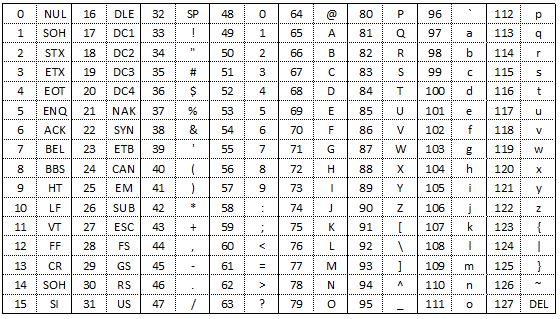
\includegraphics[width=0.24 \textwidth]{sections/ASCII-Tabelle}
\begin{tabular}{rlcrl}
	00-31:& NUL, ... & \quad & 32:& SPACE\\
	48-57:& 0-9& \quad &	65-90:& A-Z \\
	97-122:& a-z & \quad & 127:& DEL\\
\end{tabular}





	\section{Dynamische Datenstrukturen}
Man kann Speicher schon im Code definieren oder wenn benötigt wärend der Laufzeit eines Programmes Dynamisch allozieren.

\textbf{pro Memoria : Variablen}

\begin{itemize}
	\item erleichtern u.a. den Zugriff auf Speicherstellen (anstelle Adressen)  
	\item Müssen zur Entwicklungszeit im Code definiert werden
	\item Der Speicher einer Variable wird automatisch freigegeben, sobald die Variable nicht mehr gültig ist.
	
\end{itemize}

\textbf{Dynamische Speicherverwaltung}
\begin{itemize}
	\item Speicher kann zur Laufzeit (dynamisch) vom System angefordert (alloziert) werden 
	\subitem Operator: \texttt{new} (in C: Funktion \texttt{malloc()}).
	\item Dynamisch allozierter Speicher muss wieder explizit freigegeben werden
	\subitem Operator: \texttt{delete} (in C: Funktion \texttt{free()}).
	\item Dynamischer Speicher wird nicht auf dem Stack angelegt, sondern auf dem \textbf{Heap}.
	\item Auf Dynamisch allozierter Speicher kann \textbf{nur} über Pointer zugegriffen werden.
\end{itemize}

\begin{lstlisting}[mathescape]
int* pInt = new int; // Speicher für int alloziert
char* pCh1 = new char; // Speicher für char alloziert
char* pCh2 = new char;
char* pArr = new int[100]; // Array
*pInt = 23;
std::cin >> *pCh1;
pCh2 = pCh1;
// pCh2 zeigt nun auch auf die gleiche Speicherstelle wie pCh1. Damit geht aber der Zugriff auf die Speicherstelle verloren, auf die pCh2 gezeigt hat (memory leak!)
delete pInt; // Speicher freigeben
delete pCh1; // Speicher freigeben
delete pCh2; // ergibt Fehler
pInt[22] = -45; // Wert zuweisen
delete pInt; // Fehler: nur pInt[0] wird freigegeben
delete[] pInt; // korrekter Befehl
\end{lstlisting}
Beim Anwenden des \texttt{delete}-Operator auf einen bereits freigegebenen Speicherbereich, kann Probleme verursachen. Oft wird deshalb ein Pointer nach der \texttt{delete}-Operation auf 0 (bzw. \texttt{nullptr}) gesetzt.



















	\section{Structures}

Structs werden vor der main() Funktion definiert.
\begin{lstlisting}[mathescape]
struct point {
int x, y;
double gamma;
}p,q; 	// p,q schon definiert

point k; 	// Neuer "point" definieren
k.x = 2;	// Variable in struct definieren
k = {1,2,0.75} // schnell initialisieren
q = {1} $\leftrightarrow$ q ={1,0,0} // rest wird mit 0 aufgefüllt
p = q; // ist gleich wie
p.x = q.x; 
p.y = q.y;
p.gamma = q.gamma;
\end{lstlisting}

\textbf{Falsch Rekursion:} 
\begin{lstlisting}[mathescape]
struct point {int x; point y;}; // Keine Rekursion
\end{lstlisting}
\textbf{Richtig Selbstreferenzierung:} 
\begin{lstlisting}[mathescape]
struct node
{
int data;
struct node *next; // <-self reference
};
\end{lstlisting}
\textbf{Strichpunkt am Ende nicht vergessen} 
\texttt{struct point \{int i; double y;\};}

\subsection{Funktionen in Structs}
Die Konstruktor-Funktion wird bei der Generierung eines neuen Structs aufgerufen.
\begin{lstlisting}[mathescape]
struct Bar
{
	Bar() {//Konstruktor}
};
\end{lstlisting}
Funktionen können auch ausgelagert werden:
\begin{lstlisting}[mathescape]
struct Bar
{
void bier();
}bqm;
void Bar::bier() {};
\end{lstlisting}
Aufrufen der Funktion: \texttt{bqm.bier();}



























	\section{Klassen}
Eine Klasse ist eine Datenstruktur wie auch Structs. Eine Klasse hat jedoch unterschiedliche Zugriffsrechte auf die internen Variabeln, Objekte genannt.
\begin{itemize}
	\item[\texttt{private}] - (default) Elemente, meist interne Variablen, können nur innerhalb der Klasse angesprochen werden. Memeberfunktionen(Methoden) können darauf zugreifen. 
	\item[\texttt{public}] - Elemente, die meisten Methoden, können von innerhalb und ausserhalb der Klasse angesprochen werden.
	\item[\texttt{protected}] - Elemente können von innerhalb der Klasse und von abgeleiteten Klassen angesprochen werden.
\end{itemize}
\begin{lstlisting}
	class klassenname{
		private:
			int n;					//Membervariabeln
			int d;
		public:
			Klassenname(int, int);	//Konstruktor
			int f1(int);			//Memeberfunktionen (prototyp)
			void f2();
	};
\end{lstlisting}
\subsection{Konstruktoren}
Konstruktoren sind spezielle Memeberfunktionen, die den Namen der Klasse tragen. Sie können auch überladen werden und werden bei der Variabelndeklaration aufgerufen.
\begin{lstlisting}
	class rational{
		...
		public:
		rational (int num, int den);
		rational ();
	};
	rational::rational (int num, int den)
	: n(num), d(den){ //Variabeln initialisierung
		assert(den!=0); // Funktionsrumpf
	}
	rational::rational () : n(0), d(1){};
\end{lstlisting}
Damit eine Variable bereits definiert werden kann ohne ''initialisiert'' zu werden, sollte ein Default-Konstruktor erstellt werden. Dieser enthält keine Argumente setzt die Membervariablen auf ein spezifischen default-Wert. Nun kann ein Objekt vom Typ rational unterschiedlich initialisiert werden. 
\begin{lstlisting}
	rational r
	rational r1(1,2);
	rational r2 = rational(1,2);
\end{lstlisting}
Der \texttt{this->}-Pointer ist ein Pointer auf das Aktuelle Objekt.




	\section{Memory Management}
Für ein Korrektes Speichermanagement muss der neu allozierte Speicher jewils wieder in der Laufzeit des Programmes freigegeben werden.
Die Objekte welche mit \textbf{\texttt{new}} erzeugt werden leben so lange bis sie mit \textbf{\texttt{delete}} gelöst werden.
Um speicherleaks zu verhindern braucht jedes \textbf{\texttt{new}} ein entsprechendes \textbf{\texttt{delete}}!
Speicher leaks können zu heap overflow führen.
\begin{lstlisting}[mathescape]
rational* t = new rational; 
//Speicher für t wird angelegt
rational* s = t; 
//Mehrere Zeiger auf gleiches Objekt
delete s; 
//jeder Zeiger für Freigabe möglich
int nominator = (*t).denominator(); 
//Fehler: Speicher freigegeben!
\end{lstlisting}
Korrektes Memory Management kann mit klassen implementiert werden. 
Dabei soll beachtet werden das wenn Speicher im Konstruktor alloziert wird und im Destruktor freigegeben wird nicht noch andere Pointer auf das Freigegebene Objekt zeigen.
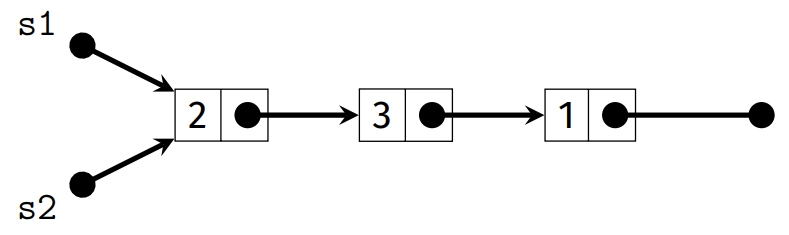
\includegraphics[width=0.24 \textwidth]{images/stack}
\begin{lstlisting}[mathescape]
stack s1;
s1.push (1);
s1.push (3);
s1.push (2);
std::cout << s1 << "\n"; // 2 3 1
stack s2 = s1;
\end{lstlisting}
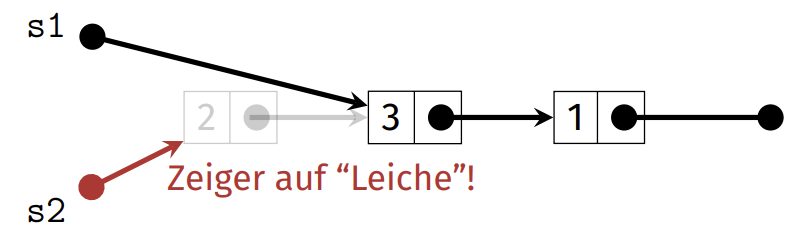
\includegraphics[width=0.24 \textwidth]{images/stack2}
\begin{lstlisting}[mathescape]
std::cout << s2 << "\n"; // 2 3 1
s1.pop ();
std::cout << s1 << "\n"; // 3 1
s2.pop (); // Programmabsturz! Pointer zeigt auf gelöschtes Objekt
\end{lstlisting}
Mögliche lösungen sind Smart-Pointer oder eine Deep-Kopie des Objektes zu erstellen.
\subsection{Smart-Pointer}
Die Idee von Smart-Pointer ist die Zeiger auf ein Objekt zu zählen und ein Objekt erst zu löschen wenn die Anzahl Pointer auf 0 fällt
\texttt{std::shared\_pointer} oder zu verhindern das mehrere Pointer auf das gleiche Objekt zeigen können \texttt{std::unique\_pointer}.
In beiden Fällen wird verhindert, dass versucht wird ein Objekt zu löschen welches schon gelöscht wurde oder noch Pointer darauf zeigen.



\subsection{Deep-Copy \& Copy Konstruktor}
Bei einer Deep-Copy oder echten Kopie eines Objektes werden alle Elemente eines Objektes Kopiert und neuem Speicher zugewiesen. 
So erhält man zwei Identische Objekte und die jeweiligen Pointer zeigen im Speicher auf zwei verschiedene Speicherabschnitte.
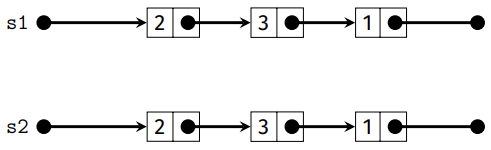
\includegraphics[width=0.24 \textwidth]{images/DeepCopy}
Dies kann mit einem Copy-Konstruktor implementiert werden. 
Der Copy-Konstruktor einer Klasse A ist erkennt man an der Deklaration \texttt{A(const A \& x);}. 
Dieser wird automatisch aufgerufen wenn Werte von Typ a initialisiert werden.
\begin{lstlisting}[mathescape]
A x = a; // a vom Typ A
A x (a);

\end{lstlisting}
Falls kein Copy-Konstruktor deklariert ist wird er automatisch erzeugt und initialisiert memberweise.
\begin{lstlisting}[mathescape]
// Coppy Konstruktor Beispiel
avec::avec(const avec& vec) : 
count(vec.count) // Init count
{	elements = new tracked[count];
	for(unsigned int i=0;i!=count;++i) 
	{
		elements[i] = vec.elements[i];
	}
}
// Destruktor Beispiel
avec::~avec() {
delete[] elements;
}
\end{lstlisting}

Das gleiche kann auch mit einer Zuweisung implementiert werden.
Dazu wird der \texttt{=} Operator überladen.
\begin{lstlisting}[mathescape]
avec& avec::operator=(const avec& t) 
{
	if (elements != t.elements) 
	// keine Selbstzuweisung
	{
		avec copy(t); // Kopierkonstruktor
		std::swap(copy.elements, elements);  
		// copy hat nun den Müll!
		std::swap(copy.count, count); 
		//copy wird aufgeräumt $\rightarrow$ Dekonstruktion
	}
	return(*this); // Rueckgabe als L-Wert (Konvention)
}
\end{lstlisting}
Ein gutes Memory Management kann im Header file erkannt werden wenn alle Fälle des Kopierens einer Klasse abgedeckt sind:
\begin{itemize}
	\item Konstruktoren
	\item Destruktoren
	\item Copy-Construktor
	\item Zuweisungsoperator
\end{itemize}
Daraus ergibt sich die Dreierregel: definiert eine Klasse eines der letzen drei, so muss sie auch die anderen zwei definieren!

\begin{lstlisting}[mathescape]
avec(unsigned int size); //Constructor
avec(const avec& vec); //Copy-Constructor
avec& operator=(const avec& vec);
//assignment operator
~avec(); //Destructor
\end{lstlisting}














	\section{Container und Iteratoren}
Container sind Datenstrukturen mit einer Ansammlungen von Elementen, auf welchen Operationen ausgeführt werden können (z.Bsp Vektor).
Die Standartbiblipthek von C++ enthält diverse Container mit unterschiedlichen Eigenschaften. \todo{Beispiele Container Eigene Section???}
Um Unterschiedliche funktionen mit Container zu realisieren (z.bsp. um diese auszugeben) sind Iterator hilfreich. Jeder C++-Container implementiert seinen eigen Iterator. Gegeben sei ein Container \texttt{c}.
\begin{tabular}{p{0.08 \textwidth}|p{0.14\textwidth}}
	\texttt{it=c.begin()} & Itarator aufs erste Element\\
	\texttt{it=c.end()} & Iterator hinters letzte Element\\
	\texttt{*it} & Zugriff aufs aktuelle Element\\
	\texttt{++it} & Iterator um ein Element verschieben\\
	\texttt{it2!=it} & (oder \texttt{==}) vergleichen von Iteratoren
\end{tabular}
Iteratoren sind eine Art Containerspezifische Zeiger. Vorteil: Nutzer müssen genaue Implementierung nicht kennen.
\begin{lstlisting}
	void print(std::vector<int> vec){
	for(std::vector<int>::iterator it= vec.begin();
		it<vec.end();
		++it){
		std::cout<<*it<<" ";
		}
	}
\end{lstlisting}
Um einen solchen Iterator zu schreiben, muss ein Klasse mit den obigen Funktionen geschreiben werden. \texttt{iterator} ist eine innere Klasse von \texttt{Container}.
\begin{lstlisting}
	class Container {
		...
		public:
		class iterator {
			...
		};
		...
	};
\end{lstlisting}
Jeder Container sollte auch ein \texttt{const\_iterator} bereitstellen. Dieser wird gebraucht, wenn nur lesezugriff gestattet ist oder das Objekt selbst \texttt{const.} ist.\\
Folgende Standard librarys gehören zu den sequenziellen container welche die daten sequentiell zugreifen.

\begin{multicols}{2}
	\textbf{Sequenzielle:}
	\begin{itemize}
		\item array
		\item vector
		\item deque
		\item forward\_list
		\item list
	\end{itemize}
	
	\textbf{Adaptors:}
	\begin{itemize}
		\item stack
		\item queue
		\item priority\_queue
	\end{itemize}
	
\end{multicols}
Container adaptoren stellen ein anderes interface für sequentielle container zu verfügung


Die Assoziativen container sind sortiert implementiert und können mit der Komplexität $O(log(n))$ durchsucht werden.
\begin{multicols}{2}
	\textbf{Assoziativ:}
	\begin{itemize}
		\item set
		\item map
		\item multiset
		\item multimap
	\end{itemize}
	
	\textbf{Assoziativ unsortiert:}
	\begin{itemize}
		\item unordered\_set
		\item unordered\_map
		\item unordered\_multiset
		\item unordered\_multimap
	\end{itemize}
\end{multicols}
Die unsortierten assoziativen container sind unsortierte (hashed) Daten Strukture welche schnell $O(1)$ (ideal) oder worst-case $O(n)$ durchsucht werden können.


	\section{Binarytrees}
Eine Liste mit jeweils 2 Nachfolgern. Dem obersten Knoten sagt man Wurzel (\textbf{root}). 
Alle Knoten (\textbf{node}) die am Ende des Baums hängen werden Blatt (\textbf{leaf}) genannt. 
Höhe eines Baums = maximale Anzahl Knoten zwischen root und leaf.
Folgendes Element links: kleiner als Knoten, rechts grösser.
\begin{lstlisting}[mathescape]
struct tNode {
	int key;
	tNode *left, *right;
};
\end{lstlisting}

Füge neuen Knoten mit Key k ein. Rekursive Methode.
\begin{lstlisting}[mathescape]
void insert(tNode *p, int k){
if(p==0{
p = new tNode;
p->key = k;
p->left = NULL; p->right = NULL;}
else if(p->key > k) insert(p->left,k);
else insert(p->right, k);}
// Aufruf:
tNode *root = NULL; insert(root,2); 
\end{lstlisting}
Iterative Methode. Rückgabewert ist ein Pointer.
\begin{lstlisting}[mathescape]
tNode* search(tNode *root, int k){
tNode *p = root;
while(p){
if(p->key == k) return p;
if(p->key > k) p = p->left;
else p = p->right;}}
//Aufruf:
tNode *x = search(root,2);
\end{lstlisting}
\todo{Binary Trees fertig machen und noch ein Beispiel dazu}

	\section{Subtyping, Polymorphie und Vererbung}
\subsection{Konzepte}
\subsubsection{Subtyping}
\begin{multicols}{2}
	Subtyping beschreibt das Konzept einer Typhirarchie. \texttt{Exp} repräsentiert Algemeine Ausdrücke. Jedes \texttt{Literal}, aber auch jede \texttt{Addition} ist ein \texttt{Exp}.\\ 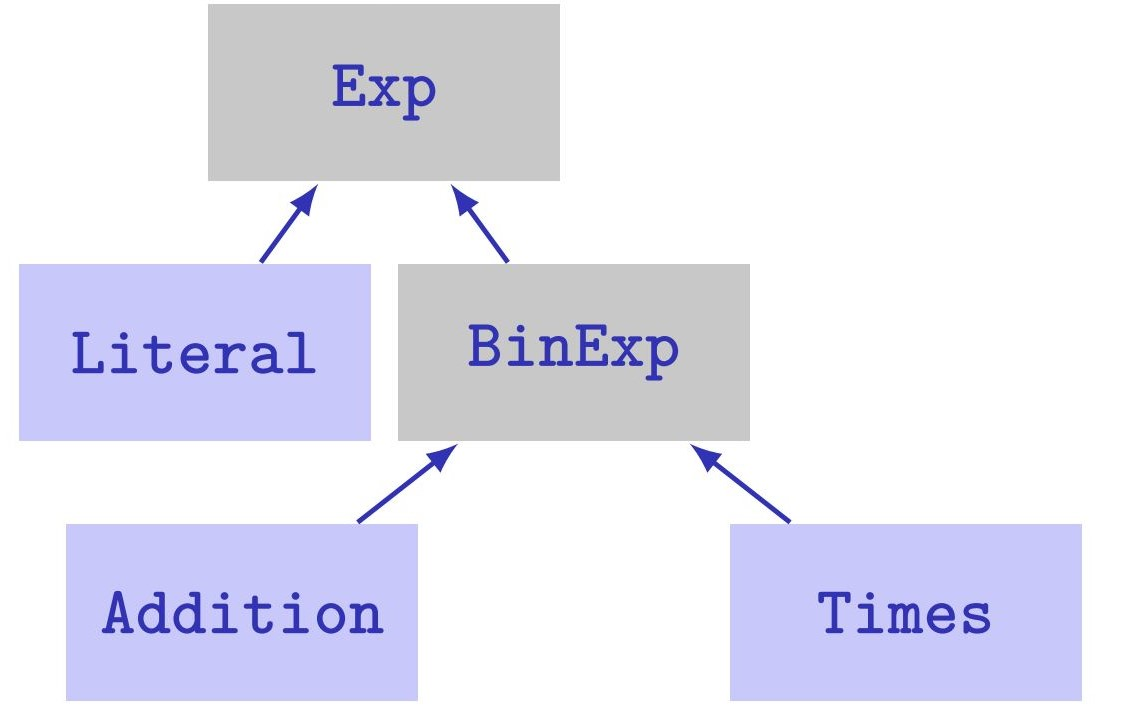
\includegraphics[width=0.12 \textwidth]{sections/subtyping}
\end{multicols}
Überall wo ein \texttt{Exp} erwartet wird, kann auch \texttt{Literal} oder \texttt{Times} genutzt werden.
\subsubsection{Polymorphie und dynamische Bindung}
Eine Variable vom statiscen Typ \texttt{Exp} kann Ausdrücke mit unterschiedlichen dynamischen Typen ''beherbergen''. Ausgeführt werden die Memeberfunktionen des dynamischen Typs.
\begin{lstlisting}
	Exp* e = new Literal(2);
	std::cout<< e->eval(); // 2
	
	e = new Addition(e,e);
	std::cout<< e->eval(); // 4 (eval von Addtion)
\end{lstlisting}
\subsubsection{Vererbung}
Manche Funktionalitäten sind für mehrere Mitglider der Typhirarchie gleich. Zum Codeduplikation zu verhindern die Funktion an Subtyp vererben.
\begin{lstlisting}
	class Exp{...};
	class BinExp : public Exp{...};
	class Times : public BinExp{...};
\end{lstlisting}
\texttt{BinExp} ist eine Subklasse von \texttt{Exp} und eine Superklasse von \texttt{Times}.
\subsection{Anwendung}
\begin{lstlisting}
	class Exp{
		public:
		virutal int size() const = 0;
		virutal double eval() const = 0;
	};
	class Literal : public Exp{
		double val;
		public:
		Literal(double v);
		int size() const;
		double eval() const;
	};
\end{lstlisting}
\texttt{Exp} ist ein abstrakte Klasse. \texttt{=0} erzwingt die Implementierung in der Subklasse. \texttt{virtual} aktiviert die Dynamische Bindung.\\
\texttt{Literal} erbt durch \texttt{public Exp} von \texttt{Exp} ist sonst aber eine normale Klasse.
Bei virtuellen Memberfunktionen bestimmt der dynamische Typ die auszuführende Memberfunktion (dynamische Bindung)  ohne virtual der statische Typ.
Gemeinsamkeiten von \texttt{Times} und \texttt{Addtion} können in \texttt{BinExp} ausgelagert werden.
\begin{lstlisting}
	class BinExp : public Exp{
		Exp* left;
		Exp* right;
		public:
		BinExp(Exp* l, Exp* r);
		int size() const;
	};
	BinExp::BinExp(Exp* l, Exp* r) : left(l), right(r) {}
	int BinExp::size() const {
		return 1 + this->left->size() + this->right->size();
	}
\end{lstlisting}
\texttt{BinExp} implementiert \texttt{eval()} nicht und ist darum auch eine abstrakte Klasse. Die Gemeinsamkeiten von \texttt{BinExp} werden weriterverwerbt.
\begin{lstlisting}
	class Addition : public BinExp {
		public:
		Addition(Exp* l, Exp* r);
		double eval() const;
	};
	Addition::Addition(Exp* l, Exp* r) : BinExp(l,r){}
	double Addition::eval() const{
		return this->left->eval() + this->left->eval();
	}
\end{lstlisting}
\texttt{Addition} erbt die Membervariabeln \texttt{left}, \texttt{right} und die Funktion \texttt{size} von \texttt{BinExp}. Genau genommen hat \texttt{Addition} jedoch kein Zugriff auf \texttt{left} und \texttt{right}, da diese \texttt{privat} sind in \texttt{BinExp}. \texttt{BinExp} bräuchte eine Memberfunktion, die \texttt{left} und \texttt{right} zurückgibt und somit den Zugriff gewährt. \todo{Das ist schon so oder???}





	\section{EBNF}
Erweiterte Backus-Naur-Form 
\begin{center}
\begin{tabularx}{\columnwidth}{|X|c|}
		\hline
\textbf{Verwendung} & \textbf{Zeichen} \\
\hline
Definition & =\\\hline
Aufzählung & ,\\\hline
Endezeichen & ;\\\hline
Alternative & |\\\hline
Option & [...]\\\hline
Optionale Wiederholung & $\left\lbrace ...\right\rbrace $ \\\hline
Gruppierung & (...)\\\hline
Anführungszeichen 1. Variante & "..."\\\hline
Anführungszeichen 2. Variante & '...'\\\hline
Komentar & (*...*)\\\hline
Spezielle Sequenz & ?...?\\\hline
Ausnahme & -\\
\hline
\end{tabularx}
\end{center}
Beispiel für einen Rechner.
Eine Zahl ist eine Folge von Ziffern. Eine Folge von Ziffern ist eine Ziffer oder eine Ziffer gefolgt von Ziffern.
\begin{lstlisting}[mathescape]
number = digits
digit = '0'|'1'|'2'|'3'|'4'|'5'|'6'|'7'|'8'|'9'
digits = digit | digit digits.

\end{lstlisting}

	\section{Library}
\subsection{Vector}
\rowcolors{2}{gray!20}{white}
\begin{center}
	\renewcommand\tabularxcolumn[1]{m{#1}}
	\begin{tabularx}{\columnwidth}{ | l  X | } 
		\hline
		v.at(pos)&access specified element with bounds checking\\
		
		v[pos] &access specified element\\
		
		v.front() &Reference to the first element\\
		
		v.back() & Reference to the last element\\
		
		v.data() & direct access to the underlying array\\
		
		v.begin()& returns an iterator to the beginning\\
		
		v.end() & returns an iterator to the end\\
		
		v.rbegin()& returns a reverse iterator to the beginning\\
		
		v.rend()& returns a reverse iterator to the end\\
		
		v.empty()& checks whether the container is empty\\
		
		v.size() & returns the number of elements\\
		
		v.max\_size()& returns the maximum possible number of elements\\
		
		v.reserve(new\_cap)& new storage is allocated\\
		
		v.capacity()& returns the number of elements that can be held in currently allocated storage\\
		
		v.shrink\_to\_fit() & reduces memory usage by freeing unused memory\\
		
		v.clear()& clears the contents\\
		
		v.insert(pos, val) &\\
		
		v.emplace(pos, args) & constructs element in-place\\ 
		
		v.erase(pos) & erases elements. v.erase(v.begin()) first element\\
	
		v.push\_back(arg) & adds an element to the end\\
	
		v.emplace\_back() & 	constructs an element in-place at the end\\
		
		v.pop\_back() & removes the last element\\
		
		v.resize(arg) & changes the number of elements stored, removes from back if smaller\\
				
		v1.swap(v2) & swaps the contents \\
		std::swap(v1, v2) & swaps the contents \\
		\hline
	\end{tabularx}
\end{center}

	\section{Examples}
\subsection{Single Linked List}
\begin{lstlisting}[mathescape]
using namespace std;
struct node
{
	int data;
	node *next;
};

class linked_list{
private:
	node *head,*tail;
public:
	linked_list(){
		head = NULL;
		tail = NULL;
	}

	void add_node(int n){
		node *tmp = new node;
		tmp->data = n;
		tmp->next = NULL;

		if(head == NULL){
			head = tmp;
			tail = tmp;
		}
		else{
			tail->next = tmp;
			tail = tail->next;
		}
	}
	
	unsigned int List::sum(){
		unsigned sum = 0;
		for (ListNode* node = first; node != sentinel; node = node->next){
			sum += node->value;
		}
		return sum;
	}
	
	void List::deleteValue(unsigned int value) {
	  if(first != sentinel)
	    {
		  auto it_old = first;
		  if(first->value == value){
			 first = first->next;
			 delete it_old;
		   }
	  else{
  		for(auto it = first->next; it != sentinel; it = it->next )
		  { 
			if(it->next->value == value && it->next != sentinel){
			  it_old = it->next;
			  it->next = it_old->next;
			  delete it_old;
			  break;}
		  }
	   }
	}
}	
};

int main()
{	linked_list a;
	a.add_node(1);
	a.add_node(2);
	return 0;
}
\end{lstlisting}


\section{Double Linked List}
\begin{lstlisting}
struct Node {
	int data;
	struct Node* next; // Ptr to next node
	struct Node* prev; // Ptr to prev node
};
\end{lstlisting}
\begin{center}
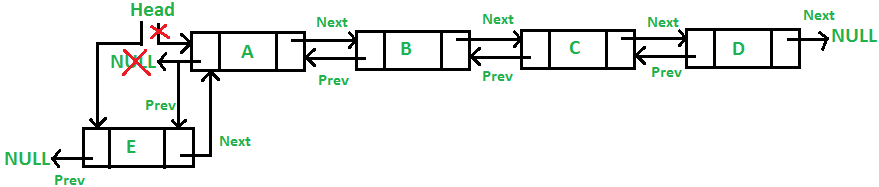
\includegraphics[width=0.24 \textwidth]{images/addFront}
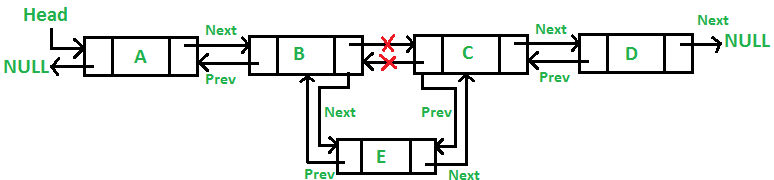
\includegraphics[width=0.24 \textwidth]{images/add_middle}
\end{center}

\begin{lstlisting}
void insertAfter(struct Node* prev_node, int new_data){
	if (prev_node == NULL) {return;}
	struct Node* new_node = (struct Node*)malloc(sizeof(struct Node));
	new_node->data = new_data;
	new_node->next = prev_node->next;
	prev_node->next = new_node;
	new_node->prev = prev_node;
	if (new_node->next != NULL)
		new_node->next->prev = new_node;
}
\end{lstlisting}
\subsection{EBNF}
Diese EBNF definition
\begin{lstlisting}
Hamburger = Bun { Onions } Patties Bun.
Patties = "P" { "P" }.
Onions = "O" "O" "O" { Onions }
Bun = "B"
\end{lstlisting}
Hat folgenden Code als umsetztung mit diesen EBNF inputs als korrekt: "BPB", "BOOOPPB", "BOOOOOOPPPPB"
\begin{lstlisting}
bool Bun(std::istream& is) {
	return consume(is, 'B'); 
	}

// Consumes next Patties = "P" { "P" }.
bool Patties(std::istream& is) {
	if (consume(is, 'P')) {
		while (lookahead(is) == 'P' && consume(is, 'P'));
		return true;
		}
	return false;
}
// Consumes next Onions = "O" "O" "O" { Onions }.
bool Onions(std::istream& is) {
	if (consume(is, 'O')) {
		unsigned int count = 1;
		while (lookahead(is) == 'O' && consume(is, 'O'))
			{++count;}
		return count % 3 == 0; // Zeigt "O" "O" "O" true
		}
	return false;
}
// Consumes next Hamburger = Bun { Onions } Patties Bun.
bool Hamburger(std::istream& is) {
	if (Bun(is)) {
		if (lookahead(is) == 'O' && !Onions(is))
			{return false;}
		if (!(Patties(is) && Bun(is)))
			{return false;}
		return !lookahead(is);
	}
	return false;
}
\end{lstlisting}


\subsection{Klassen \& Operator überschreiben}
Header file mit Klasse
\begin{lstlisting}
class Vec3 {
	public:
	Vec3() 
	: m_x(0.0f), m_y(0.0f), m_z(0.0f) {}
	
	Vec3(float x, float y, float z) 
	: m_x(x), m_y(y), m_z(z) {}
	
	// Access the vector components  
	float x() const { return m_x; }
	float y() const { return m_y; }
	float z() const { return m_z; }
	
	// Set the vector components
	void setX(float x) { m_x = x; }
	void setY(float y) { m_y = y; }
	void setZ(float z) { m_z = z; }
	
	// Compute the norm of vec
	float norm() const;
	// Return a normalized copy of a vector
	Vec3 normalized() const;
	
	// Compute the dot product between the vector and other
	float operator*(const Vec3& other) const;
	
	// Arithmetic operations with vectors
	Vec3& operator+=(const Vec3& other);
	Vec3 operator+(const Vec3& other) const;
	Vec3& operator-=(const Vec3& other);
	Vec3 operator-(const Vec3& other) const;
	
	// Arithmetic operations with scalars
	Vec3& operator/=(float scalar);
	Vec3 operator/(float scalar) const;
	Vec3& operator*=(float scalar);
	Vec3 operator*(float scalar) const;
	
	// Stream operator to display the vector's components
	// "friend" makes sure we can implement it in the class
	friend std::ostream& operator<<(std::ostream& out, const Vec3& v);
	
	// Stream operator to read the vector's components
	// "friend" makes sure we can implement it in the class
	friend std::istream& operator>>(std::istream& in, Vec3& v);
	
	private:
	float m_x;
	float m_y;
	float m_z;
};
\end{lstlisting}
.cpp File
\begin{lstlisting}
float Vec3::norm() const {
	return std::sqrt((*this) * (*this));
}

Vec3 Vec3::normalized() const {
	return (*this) / norm();
}

float Vec3::operator*(const Vec3& other) const {
	return m_x * other.m_x + m_y * other.m_y + m_z * other.m_z;
}

Vec3& Vec3::operator/=(float scalar) {
	m_x /= scalar;
	m_y /= scalar;
	m_z /= scalar;
	return *this;
}

Vec3 Vec3::operator/(float scalar) const {	Vec3 other(m_x, m_y, m_z);
	other /= scalar;
	return other;
}

Vec3& Vec3::operator*=(float scalar) {
	m_x *= scalar;
	m_y *= scalar;
	m_z *= scalar;
	return *this;
}
Vec3 Vec3::operator*(float scalar) const {
	Vec3 other(m_x, m_y, m_z);
	other *= scalar;
	return other;
}
std::ostream& operator<<(std::ostream& out, const Vec3& v) {
	return out << "[" << v.x() << ", " << v.y() << ", " << v.z() << "]";
}

std::istream& operator>>(std::istream& in, Vec3& v) {
	float x, y, z;
	char split;
	in >> std::ws;
	in >> x;
	in >> std::ws;
	in >> split;
	in >> std::ws;
	assert(split == ',');
	in >> y;
	in >> std::ws;
	in >> split;
	in >> std::ws;
	assert(split == ',');
	in >> z;
	v.setX(x);
	v.setY(y);
	v.setZ(z);
	return in;
}

Vec3& Vec3::operator+=(const Vec3& other) {
	m_x += other.m_x;
	m_y += other.m_y;
	m_z += other.m_z;
	return *this;
}

Vec3 Vec3::operator+(const Vec3& other) const {
	Vec3 sum(m_x, m_y, m_z); 
	sum += other;
	return sum;
}

Vec3& Vec3::operator-=(const Vec3& other) {
	m_x -= other.m_x;
	m_y -= other.m_y;
	m_z -= other.m_z;
	return *this;
}

Vec3 Vec3::operator-(const Vec3& other) const {
	Vec3 difference(m_x, m_y, m_z);
	difference -= other;
	return difference;
}
\end{lstlisting}
	
\end{multicols*}
\end{document}
